% !TEX encoding = UTF-8
% !TEX program = pdflatex

\documentclass[a4paper]{report}
\usepackage[T1]{fontenc}
\usepackage[utf8]{inputenc}
\usepackage[english]{babel}
\usepackage{graphicx}
\usepackage{listings}
\usepackage{xcolor}
\definecolor{light-gray}{gray}{0.95}
\lstset{language=PHP,tabsize=2,backgroundcolor=\color{light-gray}}

\begin{document}

\begin{titlepage}
\centering
\vspace*{\stretch{1}}

\includegraphics{logoRomaTre.jpg}\\
\vspace*{\stretch{6}}
{\LARGE \bf Web Services Platform for the visualization of gene expression data\par}
\vspace{0.5cm}
{\Large Comparison between differential analysis\par} 
\vspace{2cm}
di\\
{\Large \em Chiara Bartalotta, Dario Santilli, Davide Bernardini\par}
\vspace*{\stretch{2}}
\date{\currenttime}
\today
\end{titlepage}


\chapter{Usage Case}
WEB-gene expression is a platform for the visualization of gene expression data. The platform offers different services basing on the type of user. Indeed, the users are distinguished between \emph{normal user} and \emph{super user}.
\begin{itemize}
   \item \textit{super user}: super user can benefit of advanced services. he is responsible for the management of the experiments: he can insert a new experiment or delete and modify one of the instance previously stored. Furthermore, the super user is able to enable a normal user to visualize an experiment. 
   \item \textit{normal user}: after the login phase, the normal user can display only the experiments for which viewing is enabled.
\end{itemize}

\section{Super user services}

\begin{figure}[htb] 
\begin{center}
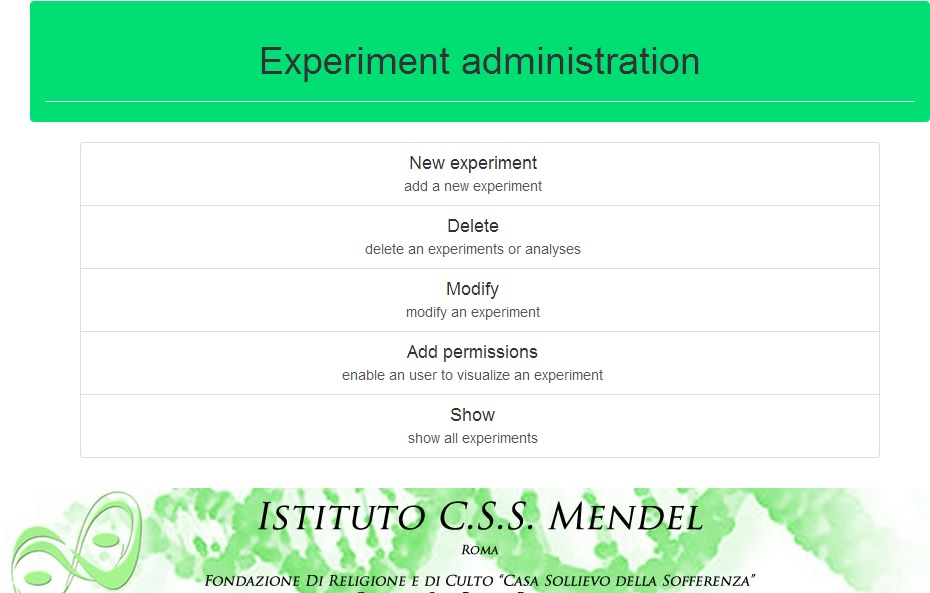
\includegraphics[scale=0.4]{figure/SUservices.jpg} 
\end{center}
\caption{Super user administration panel.}
\label{SUservices}
\end{figure}

As shown in Figure \ref{SUservices} , after the login, the platform allows the super user to access to different services. Indeed, the super user can choose among several options.

\subsection{Insert new experiment}
Through the \emph{insert} option, the user is able to store a new experiment with its relative analyses. In a first phase, the user defines the name of the new experiment, then he can choose the file with experiment's data and the system can upload it. 

\subsection{Delete and Modify}
The super user is able to delete an entire experiment stored with the option \emph{delete} and / or remove certain components analysis of the experiment, or he can only modify it. Indeed, with the \emph{modify} service, the super user can change the data of experiments. In a first phase, the user selects an existing  experiment that he want to modify, then he chooses the file with new data and the system updates the selected experiment.

\subsection{Add permission}
Another services that the platform provides to the super user  is the possibility to add permissions for the visualization of the experiments. A normal user, indeed, can see only the experiments for which he is enabled. A normal user can not visualize anything without the authorization of the super user.\\
Thought the \emph{add permission} option, the super user selects firstly the user for which to add permission and then the experiment to enable.

\section{Common service}
The main interest of the WEB-gene-expression users is to visualize the stored experiments. Therefore the primary service provided by the platform is the \emph{Show} option.\\
The 	\emph{Show} option is a common service between super user and normal user. However, a super user can visualize all the stored experiments, while a normal user can visualize only the ones for which he is enabled.

\subsection{Query}
When a user choose the \emph{show} option, he select the experiment that he want to visualize.\\
Each experiment is composed of several analyses thus the system offers the possibility to choose only the interesting ones. The two main features of each analyses are the \emph{p-value} and \emph{fold-change} values .\\
In order to shown only the analyses with user's desired characteristics, the platform provides three types of filters.

\begin{figure}[htb] 
\begin{center}
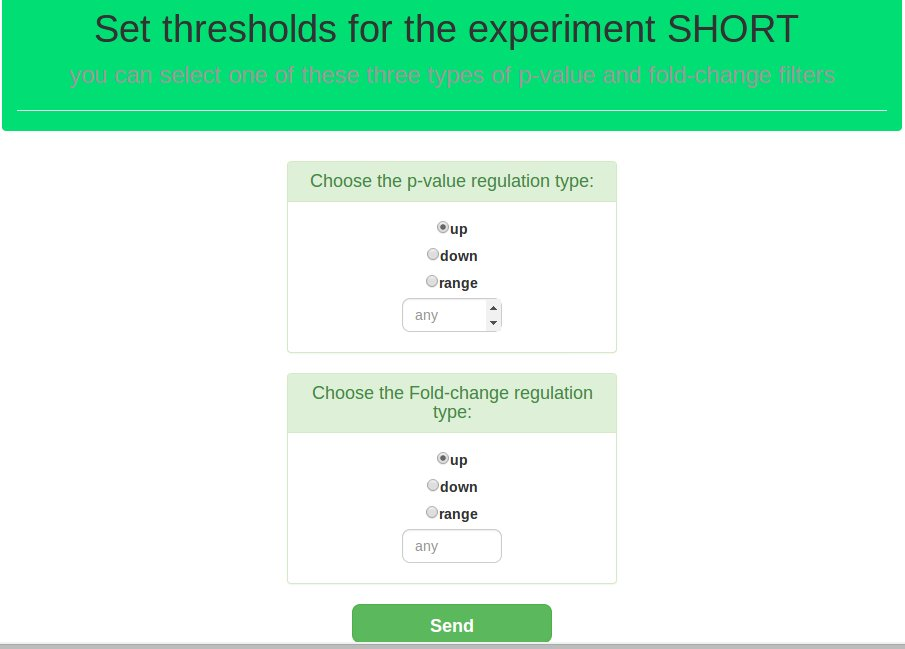
\includegraphics[scale=0.4]{figure/filters.jpg} 
\end{center}
\caption{Super user administration panel.}
\label{filters}
\end{figure}

As shown in figure \ref{filters}, the user can apply filters on the values of \emph{p-value} and \emph{fold-change}. If the user does not select a filter, the platform applies the default option and displays all the analyses without threshold on p-value and fold-change.

\begin{itemize}
    \item \textbf{p-value regulation type}: through this panel, the user can set a threshold on the p-value. Selecting \emph{up regulation}, the system will visualize the analyses with p-value greater than the specified threshold. Selecting \emph{down regulation}, the system will visualize the analyses with p-value less than the specified threshold. Finally, selecting \emph{range regulation} the system will visualize the analyses with p-value in the range of the threshold. For example, selecting \emph{range regulation} and threshold \emph{0.10} , the system shows analyses with p-value between -0.10 and +0.10.
    \item \textbf{fold-change regulation type}: analogously to the p-value regulation, the user can choose a filter on the \emph{fold-change} value. Also for the fold-change the user can define the threshold using \emph{up regulation} , \emph{down regulation} and \emph{range regulation}.
\end{itemize}

After that the user has selected a regulation option, the system shows the analyses that respect the user-defined threshold in a table.\\
As shown in figure \ref{table} , the first column of the table is the \emph{Gene} code and for each analysis there are two columns, one for the \emph{p-value} and another one for the \emph{fold-change}. The name of the analysis is specified over the p-value and fold-change field.\\

\begin{figure}[htb] 
\begin{center}
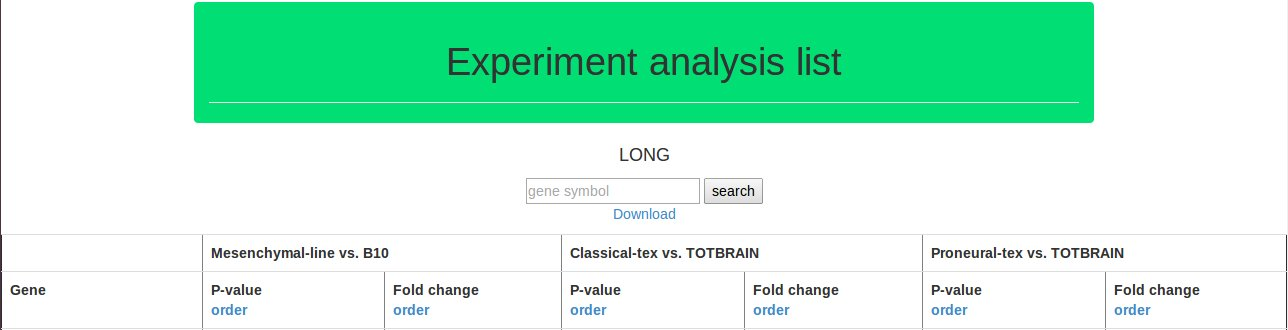
\includegraphics[scale=0.4]{figure/tableHeader.jpg} 
\end{center}
\caption{Super user administration panel.}
\label{tableHeader}
\end{figure}

The Figure \ref{tableHeader} shows that at any time the user can reorder the analyses  in ascending or descending order based on the p-value or fold-change values by clicking on \emph{order}. By specifying the \emph{Gene code} in the \emph{search bar}, the user can visualize the instance of the analyses relative to the specified gene or can visualize the instances of the analyses on the basis of a list of genes simultaneously entered in the search field and separated by a comma.\\
There is also the possibility to reset the filters that will be applied to a new table view of the same experiment with the same analyzes as selected by clicking RESET THE FILTERS.\\
The system provides the user also the possibility to download a file with the experiment data. As shown in Figure \ref{tableHeader}, the \emph{download} option is below the search field. By clicking on it, the user can save all the table in a \emph{.txt} file.


\begin{figure}[htb] 
\begin{center}
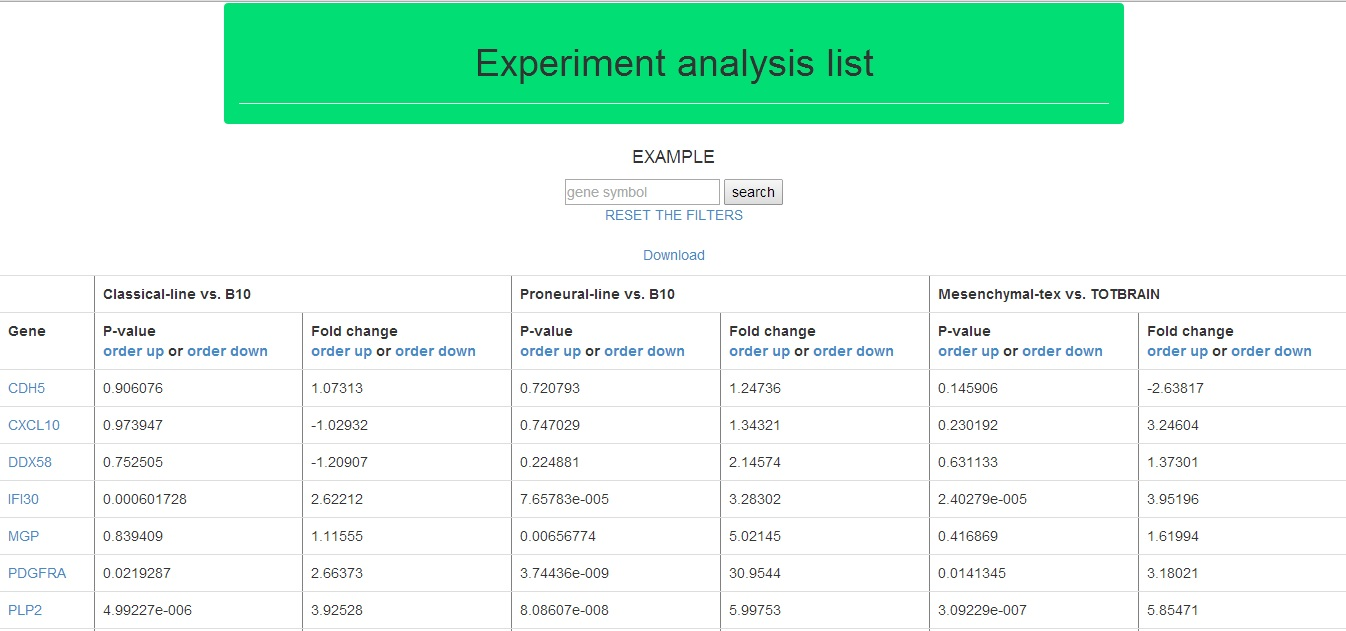
\includegraphics[scale=0.4]{figure/table.jpg} 
\end{center}
\caption{Super user administration panel.}
\label{table}
\end{figure}

\end{document}